\chapter{Ecuaciones lineales de una variable}\label{Capitulo_ecuaciones_lineales_de_una_variable}

\section{Revisión}\label{seccion_revision_ecuaciones_lineales}
Se realizará una revisión del capítulo 3 de \cite{Aops_algebra}.

\begin{ejemplo}{\ \\}
\begin{enumerate}
\item $4x=20$\\
		\textbf{Rta: }$\frac{4x}{4}=\frac{20}{4}$	
		
\item $\frac{a}{9}=\frac{2}{3}$\\
		\textbf{Rta: }
		\begin{align*}
			9\left(\frac{a}{9}\right)&=9\left(\frac{2}{3}\right)\\
			\cancel{9}\left(\frac{a}{\cancel{9}}\right)&=6\\
			a&=6
		\end{align*}

\item $-\frac{2r}{5}=12$\\
		\textbf{Rta: } 
		\begin{align*}
		\left(-\frac{5}{2}\right)\left(\-\frac{2r}{5}\right)&=	\left(-\frac{5}{2}\right)\left(12\right)\\
		r&=-30
		\end{align*}		
\end{enumerate}
\end{ejemplo}

%box de OJO, dato importante
\begin{tcolorbox}[colback=red!5!white,colframe=red!75!black]
El juego es siempre tratar dejar a la variable sola. Si ella va acompañada de un producto, por ejemplo,
\[-\frac{2f}{3}\]
debemos buscar un número que al multplicarlo por $-\frac{2}{3}$ me de $1$, y este es $-\frac{3}{2}$ pues
\[ \left(-\frac{3}{2} \right)\left(-\frac{3}{2}\right)=1 \]
\end{tcolorbox}

\begin{exer}{\ \\}
Resolver la siguientes ecuaciones
\begin{multicols}{3}
\begin{enumerate}[label=\Alph*)]
	\item $-\frac{3s}{8}=-6$
	\item $\frac{x-1}{3}=5$
	\item $3(r-5)=24$
\end{enumerate}
\end{multicols}
\end{exer}

\begin{exer}
Encontrar $a$ si $x=3$ es una solución de la ecuación $\frac{x}{a}=7$.
\end{exer}

\begin{tcolorbox}[colback=red!5!white,colframe=red!75!black]
	Otro truco es \textbf{primero simplificar la ecuación} y luego si resolver. Por ejemplo
	\[3t-7-6+2t=4t+2-6t,\]
	se puede simplificar como $5t-13=-2t-2$ y entonces $7t=11$ y así
	\[t=\frac{11}{7}\]
\end{tcolorbox}

\begin{ejemplo}{\ \\}
\begin{enumerate}
\item Encontrar los valores de $z$ que satisfacen $2z+3-4=3z-5-z$.\\
		\textbf{Rta: }Llegamos a que $-1=-5$, o sea la ecuación no es cierta! Si tenemos una igualdad que no es cierta, entonces todas las anteriores no son ciertas. Es decir, no hay solución.
\item Encontrar los valores de $r$ que satisfacen $3r+5+r=7r-2+7-3r$.
		\textbf{Rta: }Llegamos a que $4r+5=4r+5$, es decir es una igualdad que siempre es cierta independientemente de $r$! o sea hay infinitas soluciones.
\end{enumerate}
\end{ejemplo}

% box de OJO
\begin{tcolorbox}[colback=red!5!white,colframe=red!75!black]
	\begin{itemize}
	\item 	Si llegamos a una igualdad que es falsa, entonces la ecuación no tiene solución.
	\item Si llegamos a una igualdad que es siempre verdadera sin importar la variable, entonces hay infinitas soluciones.
	\end{itemize}
\end{tcolorbox}


\begin{ejemplo}
La ecuación $2x+7=3$ y $bx-10=-2$ tienen la misma solución $x$. Cuál es el valor de $b$?
\end{ejemplo}

\begin{exers}{\ \\}
\begin{enumerate}
\item Resolver las siguientes ecuaciones
		\begin{enumerate}[label=\Alph*)]
		\item $4+2,3y=1,7y-20$.
		\item $-2t+\frac{3}{2} = \frac{t}{4}-12$.
		\item $\frac{x-7}{5}=\frac{x-2}{3}$.
		\end{enumerate}
	
\item Se tiene la la ecuación $3y+2a=4y+7-y+3$.
		\begin{enumerate}[label=\Alph*)]
			\item Para qué valor de $a$ la ecuación tiene infinitas soluciones para $y$?
			\item De un valor de $a$ para el cuál la ecuación no tendría solución.
			\item Cuántos valores puede tener $a$ para que la ecuación no tenga solución.60m
		\end{enumerate}

\end{enumerate}
\end{exers}

\section{Problemas en palabras}\label{seccion_problemas_en_palabras}
La mayoría de problemas de álgebra surgen de la cotidianidad.

\begin{ejemplo}
En este momento soy 3 años mas joven que el doble de la edad que tenía hace 6 años. Cuál es mi edad en este momento?\\
\textbf{Rta: } Es simplemete la ecuación $x=2(x-6)-3$,  de donde se tiene que $x=15$.
\end{ejemplo}

\begin{exers}{\ \\}
\begin{enumerate}
\item (3.3.4 p.73 de \cite{Aops_algebra}). La profesora le dice a Carlos que reste 3 a cierto número y luego divida el resultado por 9. Sin embargo el le resta 9 y luego divide el resultado por 3, lo cual le da como resultado 43. Cuál hubiera sido su respuesta si hubiera resuelto el problema correctamente?

\item (3.3.4 p.73 de \cite{Aops_algebra}). Al final del año 1994 Walter tenía la mitad de la edad que su abuela. La suma de los años en que nacieron es 3838. Cuántos años tendrá Walter al final del año 1999?
\end{enumerate}
\end{exers}

\section{Ecuaciones lineales disfrazadas}\label{Section_ecuaciones_lineales_disfrazadas}
Resolveremos algunas ecuaciones que parece complicadas pero con un simple paso realmente son ecuaciones lineales.

\begin{ejemplo}{\ \\}
\item Encontrar todos los valores de $x$ que satisfagan la ecuación $3\sqrt{x} - 2 = 30-\sqrt{x}$.\\
		\begin{itemize}
		\item \textbf{Forma 1:} Usando una \textbf{\textit{substitución}}. Para que nos quede una ecuación lineal podemos tomar $y=\sqrt{x}$, entonces tenemos
		\[3y-2 = 30-y,\]
		de donde tenemos que $y=8$. Entonces como $y=\sqrt{x}$ entoces $8=\sqrt{x}$ y así vemos que $x=64$.
		
		\item \textbf{Forma 2:} Trabajando con $\sqrt{x}$ como una variable normal. Tenemos $4\sqrt{x}=32$ y entonces $\sqrt{x}=8$ y así calculamos que $x=64$.
		\end{itemize} 
\end{ejemplo}


% box de OJO
\begin{tcolorbox}[colback=red!5!white,colframe=red!75!black]
		Una ecuación díficil a simple vista puede ser convertida en una ecuación lineal que sabemos resolver simplemente haciendo una \textbf{sustitución}. Ejemplo, convertir
		\[3\sqrt{x} - 2 = 30-\sqrt{x},\]
		en
		\[3y-2 = 30-y\]
\end{tcolorbox}

\begin{ejemplo} Resolver la ecuación
\[\frac{3}{x} - 2=7+\frac{2}{x}\]
\begin{itemize}
	\item \textbf{Forma 1:} Para volverlo una ecuación lineal debemos deshacernos de esas $x$ en el denominador, entonces multipliquemos por $x$ la ecuación,
	\begin{align*}
		x \left( \frac{3}{x} - 2 \right) =x \left(7+\frac{2}{x}\right)\\
		\cancel{x} \frac{3}{\cancel{x}} - 2x  =7x+\cancel{x}\frac{2}{\cancel{x}}\\
		3-2x=7x+2\\
		1=9x\\
		\frac{1}{9} = x
	\end{align*}
	Es importante \textbf{comprobar }que la respuesta está bien! Hazlo!
	\item \textbf{Forma 2:} Podemos tomar una \textbf{sustitución}, por ejemplo $y=\frac{1}{x}$.
	\item \textbf{Forma 3:} Trabajando de forma normal.
\end{itemize} 
\end{ejemplo}

\begin{exers}{\ \\}
Juguemos Stop, vamos a resolver las siguientes ecuaciones el que tenga solución diferente suma más puntos.
\begin{enumerate}
\item $\sqrt[3]{2z+1} - 5 + 2 \sqrt[3]{2z+1} = -14$.
\item $2\sqrt{x} +13-\sqrt{r} = 9 - \sqrt{r}$.
\item $\frac{x}{x-1} + \frac{2}{3} = \frac{2}{x-1} $.
\end{enumerate}
\end{exers}

\newpage
\begin{exers}{\ \\}
\begin{center}
	\vspace{-5mm}
	\section*{Ejercicios de revisión}\label{section_ejercicios_ecuaciones_lineales_de_una_variable}
\end{center}
Tomado de p.82-83 de \cite{Aops_algebra}
\begin{enumerate}
\item Resolver las siguientes ecuaciones	
		\begin{multicols}{2}
		\begin{enumerate}[label=\Alph*)]
		\item $\frac{t}{3}-7+\frac{2t}{3}=-3-4$.
		\item $x-3.8x+1.1x=-4.2+2.1x+0.4$.
		\end{enumerate}
		\end{multicols}

\item Una bolsa que contiene reloes pesa 81kg. Cuando 2 relojes se quitan, el peso de la bosa baja a 73kg. La bolsa pesa 1kg cuando está vacía. Cuántos relojes quedan en la bolsa?

\item Resolver las siguientes ecuaciones	
		\begin{multicols}{2}
			\begin{enumerate}[label=\Alph*)]
				\item $\frac{2}{z}+5=\frac{5}{z} -4$.
				\item $\frac{1}{x-1} + \frac{2x}{x-1}=5$.
			\end{enumerate}
		\end{multicols}

\item Hace cinco años, mi abuelo era cinco veces mayor que lo que yo era. Dentro de tres años, mi abuelo va a ser tres veces mayor que lo que yo voy a ser. Que edad tengo en este momento?

\item Cinco enteros consecutivos son sumados. El resultado es 6 mas que el mayor de los cinco enteros. Cuál es el más pequeño de los cinco enteros?

\item Para cual valor de $b$, $x=3$ es una solución de la ecuación $bx^2+3x-2b=0$?

\item Resolver las siguientes ecuaciones	
		\begin{multicols}{2}
			\begin{enumerate}[label=\Alph*)]
				\item $\sqrt[4]{y} + \sqrt[4]{16y}-2=4$.
				\item $\frac{3}{2+\sqrt{y}} + \frac{4}{2+\sqrt{y}} = 1$.
			\end{enumerate}
		\end{multicols}
	
\item \hspace{1cm}	
	\begin{enumerate}[label=\Alph*)]
		\item Sea $x$ el número de en medio de tres enteros consecutivos. Cuál es la suma de estos tres enteros en términos de $x$?.
		\item La suma de 23 enteros consecutivos es 2323. Cuál es el mayor de estos enteros?
	\end{enumerate}

\item Resolver las siguientes ecuaciones	
		\begin{multicols}{2}
			\begin{enumerate}[label=\Alph*)]
				\item $\frac{\sqrt{3+\sqrt[3]{t}}}{\sqrt{3-\sqrt[3]{t}}} = 3$.
				\item $\frac{\sqrt{x+1}+\sqrt{x-1}}{\sqrt{x+1}-\sqrt{x-1}} = 3$.
			\end{enumerate}
		\end{multicols}
\end{enumerate}
\end{exers}
\newpage


\chapter{Mas variables}\label{Capitulo_mas_variables}
Basado en el capitulo 4 de \cite{Aops_algebra}. Al plantear expresiones a veces surge la necesidad de utilizar mas variables.

\begin{ejemplo}
	El triple de la suma de mi edad y la tuya es 4 años más que cuatro veces mi edad. Planteemos una ecuación que represente este problema\\
	\[3(x+y)=4+4x\]
	Se podrá resolver esta ecuación? Que se te ocurre hacer? Si por ejemplo al igual que cuando trabajabamos con una variable intentamos despejar $x$ nos queda
	\[3y-4=x\]
	Cúando esto es cierto? Hay solo un par de valores para los cuales es cierto? o no hay?. Si por ejemplo $x=1$, entonces $y=\frac{5}{3}$. Si $x=2$, entonces $y=2$. Hay infinitas.
\end{ejemplo}

Trabajando con varias variables nos podemos encontrar entonces con muchos tipos de expresiones como

\begin{multicols}{3}
	\begin{itemize}
		\item $\sqrt{x^2+y^2}$
		\item $2a^2b + 3b^2c + 6ac^2$
		\item $\frac{r^2+s^2}{2rs}$
	\end{itemize}
\end{multicols}

\begin{ejemplo}
	En especial, note que si tenemos un triángulo rectángulo donde un cateto mide $x$ y el otro mide $y$, entonces la expresión de cuánto mide la hipotenusa es
	\[ \sqrt{x^2+y^2} \]
\end{ejemplo}

\begin{exer}
	Si decimos que $h$ es la hipotenusa, y $c$ es uno de los catetos, cuál sería la expresión que representa la longitud del otro cateto?
\end{exer}

\begin{exer}
	Evaluar las siguientes expresiones si $a=3/2,b=1$ y $c=6$.
	\begin{multicols}{2}
		\begin{enumerate}
			\item $ab^2c$
			\item $ca^b$
			\item $a^{-1}cb$
			\item $bc^a$
		\end{enumerate}
	\end{multicols}
\end{exer}

\section{Aritmética}\label{capitulo_aritmetica_con_varias_variables}
Al igual que simplificamos expresiones de una variable, podemos simplificar expresiones de más variables.

\begin{ejemplo}
	Simplificando 
	\[
	(5x+5y+3z+3y+3x-15z+2x)
	\]
	tenemos que es lo mismo que
	\[
	10x + 8y +18z
	\]
\end{ejemplo}

\begin{ejemplo}
	Simplificando 
	\[
	\left(3ab-4cd+\frac{3}{2}\right) + \left(2cd - \frac{ab}{2} + 3\right) + (2-ab)
	\]
	tenemos que agrupar los terminos iguales $ab$ y $cd$ :
	\begin{align*}
	\left(3ab-4cd+\frac{3}{2}\right) + \left(2cd - \frac{ab}{2} + 3\right) + (2-ab) &= \left(3ab-\frac{ab}{2} -ab \right) + (2cd -4cd  ) +2 +\frac{3}{2}+ 3 && \text{Agrupando}\\
	&= \frac{6ab-ab-2ab}{2} -2cd + \frac{4+3+6}{2} \\
	&= \frac{3ab}{2}-2cd + \frac{13}{2}
	\end{align*}
	Si tuvieramos por ejemplo $cd$ y $c^2d$ no podríamos agruparlos.
\end{ejemplo}

\newpage
\begin{center}
	\vspace{-5mm}
	\addcontentsline{toc}{subsection}{Ejercicios, Mas variables: Aritmética}
	\subsection*{Ejercicios, Mas variables: Aritmética}\label{section_ejercicios_mas_variables}
\end{center}

\begin{enumerate}
	\item Cuál de las sigueintes opciones es igual a ${(2xy^2)}^5$?
	\begin{multicols}{3}
		\begin{enumerate}[label=\Alph*)]
			\item $2x^5y^{10}$
			\item $64x^6y^7$
			\item $32x^5y^{10}$
		\end{enumerate}
	\end{multicols}
	
	\item Simplificar las siguientes expresiones
	\begin{multicols}{3}
		\begin{enumerate}[label=\Alph*)]
			\item $(3rs^2)\cdot (2rs^3)$.
			\item $\sqrt[3]{27a^6b^3}$.
			\item $\frac{8x^4y^2}{x^3y^3}$.
		\end{enumerate}
	\end{multicols}
	
	\item Simplificar las siguientes expresiones
	\begin{multicols}{3}
		\begin{enumerate}[label=\Alph*)]
			\item $\frac{a}{d} + \frac{3a}{d} + \frac{2}{d} + \frac{2a-2}{d}$.
			\item $(3r^3)(2s^5)(2rs)(4r^2s^3)$.
			\item $\frac{-2x^3y^5z}{-8x^3y^2z^3}$.
		\end{enumerate}
	\end{multicols}
	
	\item Por cuál expresión debo multilicar a $2xt^3$ para obtener $32x^3t^8$?
	
	\item Escriba una expresión para la suma de $k$ enteros positivos comenzando en un entero $n$.
	
\end{enumerate}
\newpage


\section{Distribuir y Factorizar}\label{section_distribuir_y_factorizar}
\begin{tcolorbox}[colback=red!5!white,colframe=red!75!black]
	Recordemos que la \textbf{propiedad distributiva} es
	\[5(t+3s)=5t+15s.\]
	Y lo opuesto es \textbf{factorizar}, es decir 
	\[5t+15s=5(t+3s).\]
\end{tcolorbox}

\begin{ejemplo}{\ \\}
	\begin{enumerate}
		\item Expandir $3xy(x-y)$.
		\item Sacar un factor de $-15ab+35cd$.
		\item Factorizar $7r^2s^2-21rs^3+14rs^4$ 
	\end{enumerate}
\end{ejemplo}

\begin{exer}{\ \\}
	Reducir lo mayor posible la siguente expresión
	\[
	\frac{2x+4y}{8} \cdot \frac{3xy}{x^2+2xy}.
	\]
\end{exer}


Geométricamente podemos ver la factorización de la siguiente forma:
\begin{figure}[h]
	\centering
	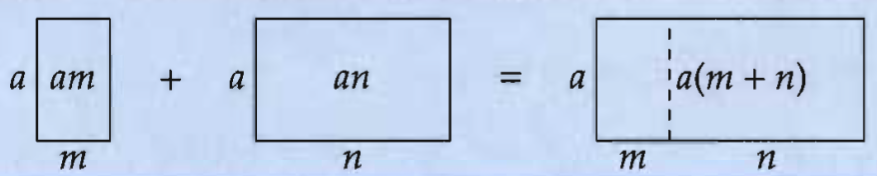
\includegraphics[width=0.7\linewidth]{Algebra/imgs/factoratimesMN}
	\caption{Visualización geométrica de la factorización y distribución.}
	\label{fig:factoratimesMN}
\end{figure}



\newpage
\begin{center}
	\vspace{-5mm}
	\addcontentsline{toc}{subsection}{Ejercicios, Mas variables: Distribuyendo y Factorizando}
	\subsection*{Ejercicios, Mas variables: Distribuyendo y Factorizando}\label{ejercicios_section_distribuir_y_factorizar}
\end{center}

\begin{enumerate}
	\item Expandir $(x+y-3z)(2x)$
	
	\item Factorizar las siguientes expresiones
	\begin{multicols}{2}
		\begin{enumerate}[label=\Alph*)]
			\item $3r^3t^2-3r^2t+7r$
			\item $-9a^3c^2+18a^2c^3-3abc$			
		\end{enumerate}
	\end{multicols}
	
	
	\item Reducir lo mayor posible la siguente expresión
	\[
	\frac{2}{3a^2-6b} \cdot \frac{9a^3-18ab}{10a^2}.
	\]
	
	\item Factorizar lo mayor posible la sguente expresión
	\[
	2x(y+1) - 6x^2(y+1)
	\]
	
	\item Expandir $(x+7)(y-4)$
	
\end{enumerate}
\newpage

\section{Fracciones}\label{section_fracciones}
\begin{ejemplo}{\ \\}
	\begin{enumerate}
		\item Simplificar como una fracción fracción
		\[
		\frac{5y}{6x^2} - \frac{4}{3xy}
		\]
		
		\item Simplificar como una fracción fracción
		\[
		\frac{2a^3}{a^3b} + \frac{3b}{a-1} - \frac{3b-3}{6ab-6a}
		\]
		\textbf{Rta: }Antes de podernos a sumar es meojor simplificar antes de buscar una fracción común.
	\end{enumerate}
\end{ejemplo}

\newpage
\begin{center}
	\vspace{-5mm}
	\addcontentsline{toc}{subsection}{Ejercicios, Mas variables: Fracciones}
	\subsection*{Ejercicios, Mas variables: Fracciones}\label{ejercicios_section_fracciones}
\end{center}

\begin{enumerate}
	\item Escribir $\frac{2}{r} + \frac{3}{s}$ como una sola fracción.
	\item Escribir $\frac{2+a}{6ab^2} + \frac{9-b}{9a^2b}$ como una sola fracción.
	\item Escribir $\frac{8r-8s}{2r^2-2rs} + \frac{3r^2}{rs-r}$ como una sola fracción.		
	
\end{enumerate}
\newpage


\section{Ecuaciones}\label{section_ecuaciones}
\begin{ejemplo}{\ \\}
	\begin{enumerate}
		\item Solucionar $x$ en la ecuación $ax=c$ en terminos de $a$ y $c$.
		
		\item Solucionar $x$ en la ecuación $ax+bc=3c-2d^2x$ en terminos de $a,b,c$ y $d$.
	\end{enumerate}
\end{ejemplo}

\newpage
\begin{center}
	\vspace{-5mm}
	\addcontentsline{toc}{subsection}{Ejercicios, Mas variables: Ecuaciones}
	\subsection*{Ejercicios, Mas variables: Ecuaciones}\label{ejercicios_section_ecuaciones}
\end{center}

\begin{enumerate}
	\item Considere la ecuación $\frac{x}{a}+b=c$.
	\begin{enumerate}[label=\Alph*)]
		\item Solucionar la ecuación para $x$ en terminos de $a,b$ y $c$.
		\item Solucionar la ecuación para $b$ en terminos de $a,c$ y $x$.
		\item Solucionar la ecuación para $a$ en terminos de $b,c$ y $x$.										
	\end{enumerate}
	
	\item Solucionar la ecuación $3xy+4=8y-2x$ para $x$ en terminos de $y$.	
	
\end{enumerate}
\newpage


\newpage
\begin{center}
	\vspace{-5mm}
	\addcontentsline{toc}{section}{Ejercicios de Revisión: Varias variables}
	\section*{Ejercicios de Revisión: Varias variables}\label{ejercicios_chapter_varias_variables}
\end{center}

\begin{enumerate}
	\item Simplificar la expresión $2a+3b+7-a+2b+5$ cuando $a=-5b$.
	
	\item Simplifique cada uno de los siuientes:
	\begin{multicols}{2}
		\begin{enumerate}[label=(\Alph*)]
			\item ${(2a^3)}^3 {(3ab^2)}^2$
			\item ${(-2c^3d)}^2 + (4cd^2)(-3c^5)$
			\item $a^3b^3 \sqrt{4a^4b^8}$
			\item $\sqrt[4]{16x^8y^4z^{16}}$
		\end{enumerate}
	\end{multicols}
	
	\item Que expresión se le debe restar a $2x-3y$ para obtener $3x+2y$?
	
	\item Exprese cada uno de los siguientes como una sola fracción:
	\begin{multicols}{2}
		\begin{enumerate}[label=(\Alph*)]
			\item $\frac{1}{a} + \frac{1}{b} + \frac{1}{c}$.
			\item $\frac{3x}{14y^2z^4} + \frac{5y}{18x^3z^2}$.
			\item $\frac{2a^2 - 4a}{3a-6} + \frac{2b^2 - 4b}{8b - 16}$.
			\item $\frac{\frac{3r^2t-6rt^2}{6r^2t^3}}{\frac{8t^3r-4t^2r^2}{6r^3t^4}}$.
		\end{enumerate}
	\end{multicols}
	
	\item Simplificar la expresión $4(x^2 -2y +7) -2(2y^2+4x+2)$ cuando $x=-y$..
	
	\item Por que fracción podemos multiplicar a $\frac{3x^3}{2y^5}$ para obtener $\frac{6y^2}{5x^2}$?
	
	\item
	\begin{enumerate}[label=(\Alph*)]
		\item Expanda el producto $(x-2)(x+2)$.
		\item Factorice la expresión $x^2-y^2$ como producto de dos expresiones tales que ninguna de estas dos es constante.
		
		\item Si $x=\frac{a}{b}$ entonces exprese $\frac{a+b}{a-b}$ en terminos de $x$.
		
		\item \textbf{Wow}. Para que valores de $a$ la ecuación $\frac{6x-a}{x-3} = 3$ no tiene solución para $x$?
		
		\item \textbf{Wow}. Para que valores de $a$ la ecuación $\frac{1}{1+\frac{1}{x}} = a$ no tiene solución para $x$?
		
	\end{enumerate}
\end{enumerate}
\newpage

\chapter{Ecuaciones lineales multivariables}\label{chapter:ecuacionesLinealesMultivaribles}

\begin{ejemplo}
	Consideremos la ecuación 
	\[
	2x-3y = 7
	\]
	Podemos intentar buscar por ensayo y error valores que funcionen. También si tenemos un valor, podemos conocer el otro (ver Tabla \ref{fig:tablaxey}).
	\begin{figure}[h]
		\centering
		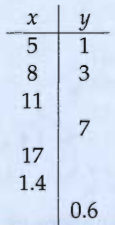
\includegraphics[width=0.2\linewidth]{Algebra/imgs/TablaProblemap105}
		\caption{Diferentes valores de $x$ e $y$.}
		\label{fig:tablaxey}
	\end{figure}
	Vemos entonces que $(5,1)$ es una solución a la ecuación. \textbf{Analizando la ecuación:} Notemos que hay un patrón lineal en la forma en que aumentan $x$ e $y$, por que?
	
	\textbf{Rta:} Si aumentamos $x$ en 3, nuestra expresión
	\[
	2x-3y
	\]
	va a aumentar 6, para compensar esto y que nos siga dando 7, tenemos que aumentar $y$ en 2, para que con el $(-3)$ me compense.
	
	Podemos tambien despejar $x$ o $y$ y reemplazar para obtener infinitas soluciones.
\end{ejemplo}

\begin{exer}
	Una solución para la ecuación $3x-5y=-1.9$ es $(x,y) = (1.2,1.1)$. Como podemos hallar otras tres soluciones de forma rápida?
\end{exer}

\section{Sustitución}\label{section:sustitucion}

\begin{ejemplo}
	Solucionar el siguiente sistema de ecuaciones
	\begin{align*}
	x+3y &= 4, \\
	-2x+5y &= -30
	\end{align*}
	Para este tipo de ecuciones podemos aplicar la \textbf{sustitución}, esto es: despejar una variable en una ecuación y reemplazarla en la otra.
\end{ejemplo}


\newpage
\begin{center}
	\vspace{-1cm}
	\addcontentsline{toc}{subsection}{Ejercicios, Ecuaciones lineales multivariables: Sustitución}
	\subsection*{ Ejercicios, Ecuaciones lineales multivariables: Sustitución}\label{ejercicios:sustitucion}
\end{center}

\begin{enumerate}
	\item Solucionar los siguientes sistemas de ecuaciones:
	\begin{multicols}{2}
		\begin{enumerate}[label=\Alph*)]
			\item \begin{align*} 2x+y&=10, \\ 3x-4y &= 37\end{align*}
			\item \begin{align*} \frac{2r}{3}+\frac{5s}{6}&=\frac{11}{2}, \\ \frac{2s}{3}&= \frac{7}{3} + \frac{r}{2}\end{align*}
		\end{enumerate}
	\end{multicols}
	\item Suponga que $x=2-t$ y que $y = 4t+7$.
	\begin{enumerate}[label=\Alph*)]
		\item Si $x=7$, a que es igual $y$?
		\item Si $x=-3$, a que es igual $y$?
		\item Encontrar $y$ en términos de $x$.
	\end{enumerate}
	
	\item En la ecuación
	\begin{align*}
	5x -6y&=1\\
	15x - 18y &= 3
	\end{align*}
	\begin{enumerate}[label=\Alph*)]
		\item Despeje $x$ de le primera ecuación y reemplacelo en la segunda. Al reemplazar, la ecuación es siempre verdadera? Que pares de números cumplen el sistema?
		
		\item Por qué el resultado de la segunda ecuación nos puede indicar que toda pareja que satisface la primera escuación también satisface la segunda?				
	\end{enumerate}
	
	\item Resolver el sistema de ecuaciones 
	\begin{align*}
	13p -92q&=273\\
	12p - 91q &= 273
	\end{align*}
\end{enumerate}
\newpage


%%%%%%%%%%%%%%%%%%%%%%%%%%%%%%%%%%%
%%%%%%%%%%%% ELIMINACIÓN %%%%%%%%%%%%%%%
%%%%%%%%%%%%%%%%%%%%%%%%%%%%%%%%%%%

\section{Eliminación}\label{section:eliminacion}

\begin{ejemplo}
	Solucionar el siguiente sistema de ecuaciones
	\begin{align*}
	2x+3y &= -11, \\
	5x-3y &= 67
	\end{align*}
	Para este tipo de ecuciones podemos aplicar la \textbf{Eliminación}, esto es: sumar las ecuaciones de forma que se eliminen variables.
\end{ejemplo}

\begin{ejemplo}
	Solucionar el siguiente sistema de ecuaciones
	\begin{align*}
	4x-7y &= 13, \\
	2x+3y &= -5
	\end{align*}
	Basta multiplicar la segunda ecuación por $(-2)$. Solución $(x,y) = (2/13, -23/13)$.
\end{ejemplo}

\begin{exer}
	Resolver los siguientes sistemas de ecuaciones
	\begin{multicols}{2}
		\begin{enumerate}[label=\Alph*)]
			\item \begin{align*} 2x+4y&=-9, \\ 2x+6y &= 7\end{align*}
			\item \begin{align*} 5x-2y&=12, \\ x-9y+22 &= -2y\end{align*}
		\end{enumerate}
	\end{multicols}
\end{exer}

\begin{ejemplo}
	Solucionar el siguiente sistema de ecuaciones
	\begin{align*}
	-u+3v &= 8, \\
	10v - 2u &= 16+4v
	\end{align*}
	
	Dividiendo por 2, tenemos entonces que ambas ecuaciones son la misma, entonces cualquier solución de una ecuación también es solucion de la otra. Entonces tenemos infinitas soluciones de $(u,v)$, como las podemos representar?
	\[
	(u,v)=?
	\]
	Entonces podemos darle a $v$ un valor cualquiera, digamos $t$, el cual llamaremos \textbf{parametro}. Entonces tenemos que las \textbf{soluciones paramétricas} son
	\[
	(u,v) = (3t-8,t)
	\]
	así vemos que son infinitas.
\end{ejemplo}

\begin{tcolorbox}[colback=black!5!white,colframe=black]
	\textbf{Aplicando a programación:}
	\begin{itemize}
		\item Para el anterior ejercicio se puede hacer graficando las rectas en geogebra, ver que son la misma.		
	\end{itemize}
\end{tcolorbox}

\begin{tcolorbox}[colback=black!5!white,colframe=black]
	\textbf{Aplicando a programación:} Puedes graficar la solución paramétrica en geogebra, una actividad con esto y mas curvas paramétricas son divertidas para que jueguen parametrizando en geogebra: \textbf{Actividad:} \url{https://www.geogebra.org/m/hhmyprpg} \textbf{Geogebra Class: }\url{https://www.geogebra.org/classroom/uct4pkgw}
\end{tcolorbox}

\begin{ejemplo}
	Solucionar el siguiente sistema de ecuaciones
	\begin{align*}
	-r+2s &= 2, \\
	-2.5r+5s &= 7
	\end{align*}
	Por un lado podemos hacr eliminación y tendríamos una igualdad falsa, entonces no habrían soluciones. Por otro lado podemos ver que ambas ecuaciones son la misma a la izquierda pero en la igualdad no son lo mismo, 
	\begin{align*}
	-5r+10s &= 5, \\
	-5r+10s &= 14
	\end{align*}
	entonces habrá alguna solución de la para este sistema? \textbf{NO!} cualquier solución de una no servirá para la otra. Entonces no hay soución (r,s).
\end{ejemplo}

\begin{exer}{\ \\}
Que valor debe tener $a$ para que hayan infinitas soluciones?
\begin{align*}
-r+2s &= 2, \\
-2.5r+5s &= a
\end{align*}
\end{exer}

\begin{tcolorbox}[colback=red!5!white,colframe=red!75!black]
	Cuando tenemos un sistema de dos ecuaciones hay tres opciones:
	\begin{itemize}
		\item \textbf{No hay solución}. Si llegamos a algo falso, por ejemplo 9=0.
		
		\item \textbf{Una solución}. 
		
		\item \textbf{Infinitas soluciones}. Si llegamos a algo siempre cierto como 0=0, o vemos que ambas ecuaciones son la misma.
	\end{itemize}
\end{tcolorbox}


\newpage
\begin{center}
	\vspace{-1cm}
	\addcontentsline{toc}{subsection}{Ejercicios, Ecuaciones lineales multivariables: Eliminación }
	\subsection*{Ejercicios, Ecuaciones lineales multivariables: Eliminación }\label{ejercicios:eliminacion}
\end{center}

\begin{enumerate}
	\item (p.117 de \cite{Aops_algebra}). Solucionar los siguientes sistemas de ecuaciones:
	\begin{multicols}{2}
		\begin{enumerate}[label=\Alph*)]
			\item \begin{align*} 3x-7y&=14, \\ 2x+7y &= 6\end{align*}
			\item \begin{align*} 5u&=-7-2v, \\ 3u &= 4v-25\end{align*}
			\item \begin{align*} \frac{2x}{13} +2y &= -2(y+1), \\ \frac{-3x}{13}&= -5(6-y)\end{align*}				
			\item \begin{align*} -2.5a +5b &=25, \\ 42+10b &= 15 + 3.75a + 4b\end{align*}				
		\end{enumerate}
	\end{multicols}
	
	\item (p.117 de \cite{Aops_algebra}). Describa todas las soluciones de cada uno de los siguientes sistemas de ecuaciones
	\begin{multicols}{2}
		\begin{enumerate}[label=\Alph*)]
			\item \begin{align*} 2x+3y&=7, \\ 14x &= 49 - 21y\end{align*}
			\item \begin{align*} \frac{3x}{5} - \frac{4y}{5} &= 3, \\ 8y-6x &=5\end{align*}		
		\end{enumerate}
	\end{multicols}
	
	\item Para que valor de de la constante $a$, el siguiente sistema de ecuaciones tiene infinitas soluciones ?
	\begin{align*}
	2x + 5y&= -8\\
	6x &= 16 + a - 15y
	\end{align*}
	
	\item (p.117 de \cite{Aops_algebra}). (\textbf{WOW}). Para que valores de las constantes $a,b,c,d$ y $e$, el siguiente sistema de ecuaciones tiene infinitas soluciones ?
	\begin{align*}
	ax+by&=d\\
	ax+cy&=e
	\end{align*}
\end{enumerate}
\newpage

%%%%%%%%%%%%%%%%%%%%%%%%%%%%%%%%%%%
%%%%%%%% PROBLEMAS DE PALABRAS  %%%%%%%%%%%
%%%%%%%%%%%%%%%%%%%%%%%%%%%%%%%%%%%

\section{Problemas en palabras y mas ecuaciones disfrazadas}\label{section:problemasEnPalabrasyEcuacionesDisfrazadas}

\begin{ejemplo}{\ \\}
	Se jugó un partido de basketball entre dos equipos, Bucaros y Arrieros. Los dos equipos marcaron en total 34 puntos, y los Bucaros ganaron por un margen de 14 puntos. Cuántos puntos marcaron los Arrieros?
	
	\textbf{Solución: }Importante elegir bien el nombre de las variables: ''b`` y ''a`` para el total de puntos maracos por los Bucaros y el total marcado por los Arrieros respectivamente. 
	\begin{align*}
	b + a&= 34\\
	b-b &= 14
	\end{align*}
	Podemos sumar las ecuaciones y resolver facilmente.
\end{ejemplo}

\begin{ejemplo}{\ \\}
	El peso de Juan y dos veces el de Marcos es 361kg y el peso de Marcos y dos veces el de Juan es 362kg. Cuánto pesan Juan y Marcos juntos?
	
	\textbf{Solución: }
	\begin{align*}
	j + 2m&= 361\\
	2j+m &= 362
	\end{align*}
	Sumando, $3j+3m=723$, entonces $j+m=241$.
	\begin{align*}
	b + a&= 34\\
	b-b &= 14
	\end{align*}
	Podemos sumar las ecuaciones y resolver facilmente.
\end{ejemplo}

\begin{ejemplo}{\ \\}
	Hace dos años, Germán tenía nueve veces la edad de Carol. El ahora tiene 7 veces la edad de ella. Cuántos años tienen que pasar desde ahora para que Germán tenga cinco veces la edad de Carol?	
	\textbf{Solución: }
	\begin{align*}
	g&= 7c\\
	g-2 &= 7(c-2)
	\end{align*}
	Sustituyendo $g=7c$, encontramos que $c=8$ y por tanto $g=56$. Para responder la pregunta podemos crear una nueva variable: $t$
	\[56+t = 5(8+t)\]
	de donde tenemos que deben pasar $t=4$ años.
\end{ejemplo}

\begin{exer}{\ \\}
	5 pelotas verdes y dos rojas pesan juntas 10kg, y una pelota verde y 4 rojas pesan juntas 7kg. Si todas las bolas rojas pesan la misma cantidad y todas las verdes pesan lo mismo, cuánto es el peso de 8 pelotas rojas y 8 verdes?
\end{exer}

\begin{exer}{\ \\}
	En cierto momento, Juana nota que su reloj digital marca las dos de la tarde y $a$ minutos. Quince minutos mas tarde el reloj marca las tres y $b$ minutos. Ella se asombra al darse cuenta que $a$ es seis veces mas grande que $b$. Que hora era cuando ella vió el reloj por segunda vez?
\end{exer}

\begin{ejemplo}{\ \\}
	Encontrar todos los posibles valores de $a$ y $b$ tales que la suma de sus raices cuadradas sea 37 y la raiz cuadrada de $a$ sea 10 mas que el doble de la raiz de $b$.
	
	\textbf{Solución: }
	\begin{align*}
	\sqrt{a} + \sqrt{b}&= 37\\
	\sqrt{a}&= 2\sqrt{b}+10
	\end{align*}
	Podemos continuar solucionandolo así. Pero que sería mas sencillo solucionar
	\begin{align*}
	r + s= 37\\
	r &= 2s+10
	\end{align*}
	Teniamos entonces una ecuacion lineal disfrazada. De donde obtenemos $r=28$ y $s=9$, entonces $a=28^2$ y $b=9^2$.
\end{ejemplo}

\begin{ejemplo}{\ \\}
	Encontrar todas las parejas $(x,y)$ que satisfacen la siguiente ecuación
	\begin{align*}
	\frac{3}{x} - \frac{2}{y} &= -\frac{7}{2}\\
	\frac{6}{x} + \frac{4}{y} &= 9
	\end{align*}
	
	\textbf{Solución 1: }
	Para deshacernos de los denominadores,
	\begin{align*}
	2xy \left( \frac{3}{x} - \frac{2}{y} \right) &= 2xy\left( -\frac{7}{2} \right)\\
	xy \left( \frac{6}{x} + \frac{4}{y} \right) &= xy\left( -9 \right)
	\end{align*}
	Entonces tenemos
	\begin{align*}
	-4x+6y&=-7xy \\
	4x+6y&=9xy
	\end{align*}
	sumando tenemos $12y=2xy$, podemos dividir por $y$? Si! pues $y$ no puede ser cero. Entonces $x=6,y=1/2$.
	
	\textbf{Solución 2: }
	Para evitar trabajar con los reciprocos $1/x$ y $1/y$ podemos usar otras variables para ellos, $r$ y $s$ respectivamente, entonces
	\begin{align*}
	3r -2s&=  -\frac{7}{2} \\
	6r + 4s &= -9 
	\end{align*}
	este sistema es mucho mas fácil y podemos encontrar la solución $(r,s)=(1/6,2)$, entonces $(x,y)=(6,1/2)$.
	
	\textbf{Solución 3: }
	Si te detienes un poco a pensar puede ver que multiplicando la primera ecuación por 2 nos deja $-4/y$ en la primera y $4/y$ en la segunda,
	\begin{align*}
	\frac{6}{x} - \frac{4}{y} &= -7\\
	\frac{6}{x} + \frac{4}{y} &= 9
	\end{align*}
	sumando tenemos $12/x = 2$, entonces $x=6$.		
\end{ejemplo}

\newpage
\begin{center}
	\vspace{-1cm}
	\addcontentsline{toc}{subsection}{Ejercicios, Ecuaciones lineales multivariables: Problemas en palabras y mas ecuaciones disfrazadas }
	\subsection*{Ejercicios, Ecuaciones lineales multivariables: Problemas en palabras y mas ecuaciones disfrazadas.}\label{ejercicios:part:algebra:chapter:problemasEnPalabrasyEcuacionesDisfrazadas}
\end{center}	
\begin{enumerate}
	\item (p.125 \cite{Aops_algebra}). Resolver el sistema de ecuaciones para $x$ e $y$.
	\begin{align*}
	\frac{6}{x} + \frac{7}{y} &= 4\\
	\frac{2}{x} -  \frac{5}{y} &= 16
	\end{align*}
	\item (p.126 \cite{Aops_algebra}). La suma de las areas de dos cuadrados es 65, mientras que la diferencia en sus areas es 33. Encontrar la suma de sus perimetros
	
	\item (p.126 \cite{Aops_algebra}). \textbf{Wow}. Encontrar $r$ y $s$ si $\sqrt[3]{r}+ 9\sqrt{s} =21$ y $10 \sqrt[3]{r} - \sqrt{s} =28$
	
\end{enumerate}
\newpage

%%%%%%%%%%%%%%%%%%%%%%%%%%%%%%%%%%%
%%%%%% PROBLEMAS DE MAS VARIABLES  %%%%%%%%%%
%%%%%%%%%%%%%%%%%%%%%%%%%%%%%%%%%%%

\section{Problemas con mas variables }\label{section:problemas_con_mas_variables}

\begin{ejemplo}{\ \\}
	Resolver el sistema de ecuaciones
	\begin{align*}
	x+3y-4z &= 25\\
	-2x+5y+7z &= -66\\
	3x-2y+3z &= 7
	\end{align*}
	\textbf{Solución: }Tratemos de convertirlo en un problema que conozcamos. De la primera ecuación $x=25-3y+4z$ podemos reemplazarla en las otras dos para solucionar y poder calcular $y$ e $z$. De donde podemos calcular $y=-2$, $z=-6$ y con esto podemos calcular $x$, que sería $7$. Entonces la solución es $(x,y,z) = (7,-2,-6)$.
\end{ejemplo}

\begin{tcolorbox}[colback=red!5!white,colframe=red!75!black]
	\textbf{Sustituir} es una herramienta útil para solucionar problemas con muchas variables.
\end{tcolorbox}

\begin{ejemplo}{\ \\}
	Resolver el sistema de ecuaciones
	\begin{align*}
	2x-3y+6z &= -12\\
	5x+2y-8z &= 29\\
	7x+6y+4z &= 49
	\end{align*}
	\textbf{Solución: } Aquí no podemos sustituir sin involucrarnos con fracciones, lo cual es un poco incómodo. Podemos entonces eliminar la variable que queramos,
	\begin{align*}
	4x-6y+12z &= -24 \quad \text{multiplicamos por 2}\\
	15x+6y-24z &= 87 \quad \text{multiplicamos por 3}\\
	7x+6y+4z &= 49
	\end{align*}
	de las primera dos ecuaciones tenemos $19x-12z=63$ y de la primera y tercera $11x +16z=25$. Redujimos entonces el problema a
	\begin{align*}
	19x-12z &= 63\\
	11x +16z &= 25
	\end{align*}
	De acá nuevamente eliminando, podemos encontrar $x=3$ y $z=-1/2$. Entonces la solución es $(x,y,z) = (3,5,-1/2)$.	
\end{ejemplo}

\begin{ejemplo}{\ \\}
	En la tienda de las vocales, cada vocal se vende a diferente precio, pero todas las consonantes son gratis. La palabra ``triangle'' se vende a $\$ 6$, ``square'' a $\$ 9$, ``pentagon'' a $\$ 7$, ``cube'' a $\$ 7$ y ``tetrahedron'' a $\$8$. Cuánto cuesta la palabra ``octahedron''?
	\textbf{Solución: } 
	\begin{align*}
	a+e+i &= 6\\
	a+e+u &= 9\\
	a+e+o &= 7\\
	e+u &= 7 \\
	a+2e+o &= 8
	\end{align*}
	De la segunda y cuarta ecuación tenemos que $a=2$. Entonces ahora tenemos
	\begin{align*}
	e+i &= 4\\
	e+u &= 7\\
	e+o &= 5\\
	2e+o &= 6
	\end{align*}
	Restanto la segunda ecuación de la cuarta, tenemos $e=1$, y con esto ya podemos saber el valor de las otras vocales: $i=3,u=6$ y $o=4$. Entonces la solución de las ecuaciones es $(a,e,i,o,u) = (2,1,3,4,6)$.Y por tanto ``octahedron'' cuesta $\$ 11$.
\end{ejemplo}

\newpage

\begin{center}
	\vspace{-1cm}
	\addcontentsline{toc}{subsection}{Ejercicios, Ecuaciones lineales multivariables:Problemas con mas variables. }
	\subsection*{ Ejercicios, Ecuaciones lineales multivariables:Problemas con mas variables.}
\end{center}	
\begin{enumerate}
	\item (p.130 \cite{Aops_algebra}). Encontrar todas las soluciones del siguiente sistema de ecuaciones 
	\begin{align*}
	x+3y+2z &= 6\\
	-3x+y+5z &= 29\\
	-2x-3y+z &= 14
	\end{align*}
	
	\item (p.131 \cite{Aops_algebra}). Encontrar todas las soluciones del siguiente sistema de ecuaciones 
	\begin{align*}
	2x-5y+3z &= 25\\
	-x-y+4z &= -6\\
	3x + 3y -z &= -4
	\end{align*}
	
	\item (p.131 \cite{Aops_algebra}). En el cuadrado mágico que se muestra en la Figura \ref{fig:cuadrado_magico}, la suma de los números en cada fila, columna y diagonal es la misma. Encontrar el valor de $y+z$
	\begin{figure}[H]
		\centering
		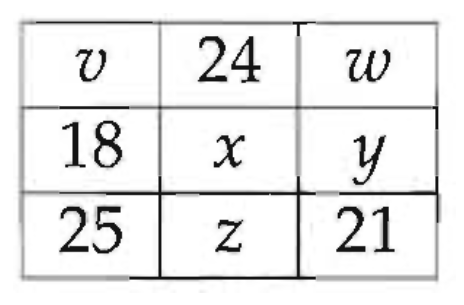
\includegraphics[width=0.25\linewidth]{Algebra/imgs/cuadrado_magico.png}
		%\caption{_caption_}
		\label{fig:cuadrado_magico}
	\end{figure}
	
	\item (p.131 \cite{Aops_algebra}). 	Considere el siguiente sistema de ecuaciones
	\begin{align*}
	2a+3b-4c &= 7\\
	a-b+2c &= -6
	\end{align*}
	\begin{enumerate}[label=(\Alph*)]
		\item Encontrar una solución $(a,b,c)$ que satisfaga ambas ecuaciones.
		\item Puede encontrar usted otra tripleta $(a,b,c)$ que satisfaga ambas ecuaciones?
		\item Solucionar $b$ en términos de $a$ y $c$ en terminos de $a$. Cuántas soluciones tiene este sistema?
	\end{enumerate}
	
\end{enumerate}
\newpage


\newpage
\begin{center}
	\vspace{-5mm}
	\addcontentsline{toc}{section}{Ejercicios derevisión: Ecuaciones lineales multivariables}
	\section*{Ejercicios de revisión: Ecuaciones lineales multivariables }\label{section:label_section}
\end{center}

\begin{enumerate}
	\item (p.133 \cite{Aops_algebra}). Encuentre tres parejas $(a,b)$ que satisfagan la ecuación $3a-5b=9$.
	
	\item (p.133 \cite{Aops_algebra}).Utilice \textbf{sustitución} para resolver el siguiente sistema de ecuaciones
	\begin{align*}
	x+4y &= -5\\
	3x-8y&=45
	\end{align*}
	
	\item (p.133 \cite{Aops_algebra}).Utilice \textbf{sustitución} para resolver el siguiente sistema de ecuaciones
	\begin{align*}
	3a-b&= 11\\
	6a+4b&=1
	\end{align*}
	
	\item (p.133 \cite{Aops_algebra}).Utilice \textbf{eliminación} para resolver el siguiente sistema de ecuaciones
	\begin{align*}
	5x-6y &= -64\\
	7x+3y&= -44
	\end{align*}
	
	\item (p.133 \cite{Aops_algebra}).Utilice \textbf{eliminación} para resolver el siguiente sistema de ecuaciones
	\begin{align*}
	3x-8y &= -7\\
	6x+16y&= 4
	\end{align*}
\end{enumerate}
\newpage